\documentclass[aspectratio=169]{beamer}

\usepackage[french]{babel}
\usepackage[utf8]{inputenc}
\usepackage[T1]{fontenc}
\usepackage{lmodern}
\usepackage{graphicx}
\usepackage{amsmath}
\usepackage{hyperref}

% =======================
% Thème "Underwater" (resources/templates/beamerthemeUnderwater.sty)
% =======================
\usepackage[showclublogo, transparentlogo]{beamerthemeUnderwater}

\ffessmlogo{images/logo_ffessm}
\clublogo{images/logo_cst}

% Palette FFESSM partagée (emphase inline dans le contenu des slides)
% Palette de couleurs FFESSM partagée par les cours théoriques, pour un
% usage en emphase inline dans le contenu des slides (ex: \textcolor
% {ffessmred}{...}). Indépendante du thème beamer (Underwater) : ce sont
% des couleurs de contenu, pas de template visuel.
\definecolor{ffessmblue}{RGB}{0,70,140}
\definecolor{ffessmlight}{RGB}{220,235,247}
\definecolor{ffessmred}{RGB}{190,30,45}
\definecolor{ffessmdarkblue}{RGB}{0,55,110}


% =======================
% Infos titre
% =======================
\title[Formation théorique N1]{Formation Théorique N1}
\subtitle{Cours Niveau 1 — Découverte et sécurité en plongée}
\author[Théo NASSOUR]{Théo NASSOUR\\\small Stagiaire MF1}
\institute[CST]{CST — Club Subaquatique Thiernois}
\date[]{\today}

% Pour avoir un peu plus d'espace
\setlength{\parskip}{4pt}

% Pour afficher la table des matières à chaque début de section
% (snippet partagé par tous les cours théoriques)
% Rappel du plan (section courante) affiché automatiquement à chaque
% nouvelle section. Partagé par tous les cours théoriques (n1/n2/n3) —
% convention de structure de document, indépendante du thème visuel.
\AtBeginSection[]
{
  \begin{frame}
    \frametitle{Table des matières}
    \tableofcontents[currentsection]
  \end{frame}
}


\begin{document}

% Page de titre (snippet partagé par tous les cours théoriques)
% Page de titre — partagée par tous les cours théoriques (n1/n2/n3).
\begin{frame}[plain]
  \titlepage
\end{frame}


% Table des matières
\begin{frame}{Plan du cours}
  \tableofcontents
\end{frame}

% =======================
% Inclusion des slides
% =======================

\section{Introduction et objectifs}

\begin{frame}{Pourquoi la plongée ?}
  \begin{itemize}
    \item La mer : un monde \textbf{merveilleux et mystérieux}.
    \item Découvrir de nouvelles sensations et un \textbf{nouveau mode de communication}.
    \item Apprendre à \textbf{maîtriser son corps} dans un milieu liquide.
    \item La plongée reste un \alert{plaisir} à condition de respecter quelques principes.
  \end{itemize}
\end{frame}

\begin{frame}{Rôle de la formation théorique}
  \begin{itemize}
    \item Acquérir des \textbf{connaissances pratiques et théoriques} adaptées au N1.
    \item Comprendre les \textbf{phénomènes physiques} qui agissent sur le plongeur.
    \item Connaître et appliquer les \textbf{règles de sécurité}.
    \item Savoir reconnaître les \textbf{dangers du milieu} et adopter la bonne attitude.
  \end{itemize}
\end{frame}

\begin{frame}{Objectifs du cours}
  À l’issue de ce cours, le plongeur Niveau 1 devra :
  \begin{itemize}
    \item Situer son niveau dans l’\textbf{organisation fédérale} (FFESSM/CMAS).
    \item Expliquer simplement la \textbf{pression} et la \textbf{loi de Boyle-Mariotte}.
    \item Comprendre la \textbf{flottabilité} et l’utilisation du lest et du gilet.
    \item Identifier les principaux \textbf{accidents barotraumatiques} et leurs préventions.
    \item Comprendre la \textbf{surpression pulmonaire} et l’\textbf{accident de décompression}.
    \item Connaître les \textbf{dangers du milieu} et les \textbf{règles de sécurité}.
  \end{itemize}
\end{frame}

\begin{frame}{Présentation du CST}
  \begin{itemize}
    \item Club associatif affilié à la \textbf{FFESSM}.
    \item Encadrement : E1, E2, E3 / MF1, E4 / MF2.
    \item Formation pratique et théorique vers les \textbf{niveaux fédéraux}.
    \item Sorties, entraînements, et \textbf{esprit de club}.
  \end{itemize}
\end{frame}

\section{Organisation fédérale et prérogatives}

\begin{frame}{La FFESSM}
  \begin{itemize}
    \item \textbf{Fédération Française d’Études et de Sports Sous-Marins}.
    \item Seule fédération reconnue par l’État pour :
          \begin{itemize}
            \item définir les \textbf{règles techniques et administratives},
            \item organiser les \textbf{compétitions} subaquatiques.
          \end{itemize}
    \item Regroupe les clubs associatifs et leurs licenciés.
    \item La licence permet : formations, brevets, assurance plongée, etc.
  \end{itemize}
\end{frame}

\begin{frame}{La CMAS}
  \begin{itemize}
    \item \textbf{Confédération Mondiale des Activités Subaquatiques}.
    \item Réunit des fédérations de nombreux pays.
    \item Objectifs : développer la connaissance et la protection du monde subaquatique,
          favoriser les sports subaquatiques.
    \item Votre Niveau 1 FFESSM correspond à une \textbf{étoile CMAS},
          reconnu dans de nombreux pays.
  \end{itemize}
\end{frame}

\begin{frame}{Prérogatives du plongeur Niveau 1}
  \begin{itemize}
    \item Accès à l’\textbf{espace médian} : jusqu’à \textbf{20 m}.
    \item Toujours \textbf{accompagné} par un guide au minimum Niveau 4.
    \item Aucune compétence d’\textbf{autonomie}, sauf pour ceux qui sont \textbf{PA12}.
  \end{itemize}

  \begin{block}{Conditions administratives}
    \begin{itemize}
      \item Certificat médical de non contre-indication (moins d’un an).
      \item Licence FFESSM en cours de validité.
      \item Passeport ou carte CMAS.
      \item Carnet de plongée.
      \item Autorisation parentale si mineur.
    \end{itemize}
  \end{block}
\end{frame}

\section{Pressions et loi de Boyle-Mariotte}

\begin{frame}{Qu’est-ce que la pression ?}
  \begin{block}{Définition}
    La pression est une \textbf{force exercée perpendiculairement} sur une surface.\\[4pt]
    \[
      P = \frac{F}{S}
    \]
    avec $P$ en bar, $F$ en newton (ou kg) et $S$ en cm\textsuperscript{2}.
  \end{block}

  \begin{itemize}
    \item Unité pratique en plongée : \textbf{bar}.
    \item 1 bar $\approx$ 1 kg/cm\textsuperscript{2}.
  \end{itemize}
\end{frame}

\begin{frame}{Pression atmosphérique}
  \begin{itemize}
    \item La Terre est entourée d’une \textbf{couche d’air} : l’atmosphère.
    \item Le poids de cette atmosphère exerce une pression sur tous les corps.
    \item À la surface de la mer, on considère :
          \[
            P_{\text{atm}} = 1 \text{ bar}
          \]
  \end{itemize}
\end{frame}

\begin{frame}{Pression hydrostatique (relative)}
  \begin{columns}[c]
    \begin{column}{0.62\textwidth}
    \begin{itemize}
      \item Colonne d’eau de 10 m de haut sur 1 cm\textsuperscript{2} :
            \begin{itemize}
              \item Volume = 1 dm\textsuperscript{3} = 1 L $\Rightarrow$ masse $\approx 1$ kg.
              \item $\Rightarrow P = 1$ bar.
            \end{itemize}
      \item \textbf{Règle pratique :} la pression augmente de \textbf{1 bar tous les 10 m}.
      \item À 20 m : $P_{\text{eau}} = 2$ bar, à 30 m : 3 bar, etc.
    \end{itemize}
    \end{column}

    \begin{column}{0.38\textwidth}
      \centering
      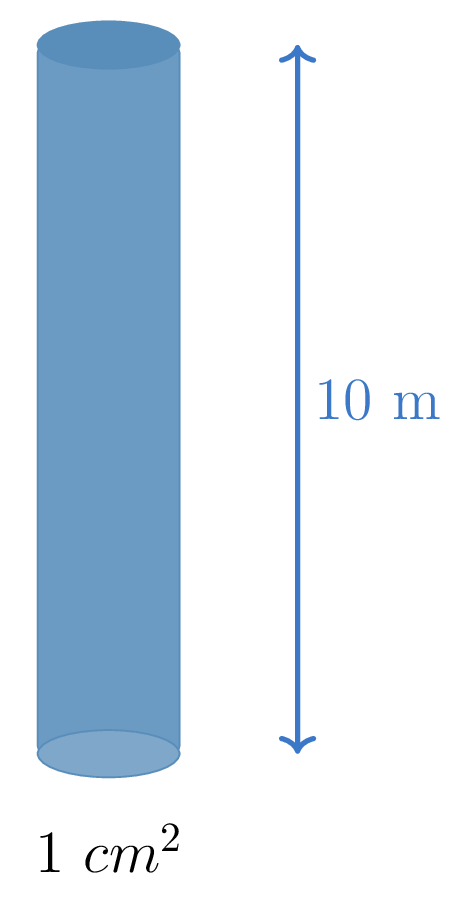
\includegraphics[height=0.6\textheight]{images/colonne_pression}
    \end{column}
  \end{columns}
\end{frame}

\begin{frame}{Pression absolue}
  \begin{block}{Définition}
    \[
      P_{\text{abs}} = P_{\text{atm}} + P_{\text{hydro}}
    \]
  \end{block}

  \begin{itemize}
    \item Surface : $P_{\text{abs}} = 1$ bar.
    \item 10 m : $P_{\text{abs}} = 1 + 1 = 2$ bar.
    \item 20 m : $P_{\text{abs}} = 1 + 2 = 3$ bar.
    \item 30 m : $P_{\text{abs}} = 1 + 3 = 4$ bar.
    \item 40 m : $P_{\text{abs}} = 1 + 4 = 5$ bar.
  \end{itemize}
\end{frame}

\begin{frame}{Loi de Boyle-Mariotte}
  \begin{block}{Énoncé}
    Pour une quantité de gaz donnée à température constante :
    \[
      P \times V = \text{constante} \quad \Rightarrow \quad P_1 V_1 = P_2 V_2
    \]
  \end{block}

  \begin{itemize}
    \item Le corps humain contient :
          \begin{itemize}
            \item des \textbf{solides} (os) et des \textbf{liquides} (sang), \alert{incompressibles},
            \item des \textbf{gaz} (poumons, sinus, oreilles, tube digestif), \alert{compressibles}.
          \end{itemize}
    \item Les volumes d’air \textbf{diminuent à la descente} et \textbf{augmentent à la remontée}.
  \end{itemize}
\end{frame}

\begin{frame}{Exemple simple}
  \begin{columns}[c]
    \begin{column}{0.6\textwidth}
      \begin{itemize}
        \item Ballon d’1 L en surface ($P = 1$ bar).
        \item À 10 m ($P = 2$ bar) :
              \[
                1 \times 1 = 2 \times V_2 \Rightarrow V_2 = 0{,}5 \text{ L}
              \]
        \item À 20 m ($P = 3$ bar) :
              \[
                1 \times 1 = 3 \times V_3 \Rightarrow V_3 \approx 0{,}33 \text{ L}
              \]
      \end{itemize}
    \end{column}
    \begin{column}{0.4\textwidth}
      \centering
      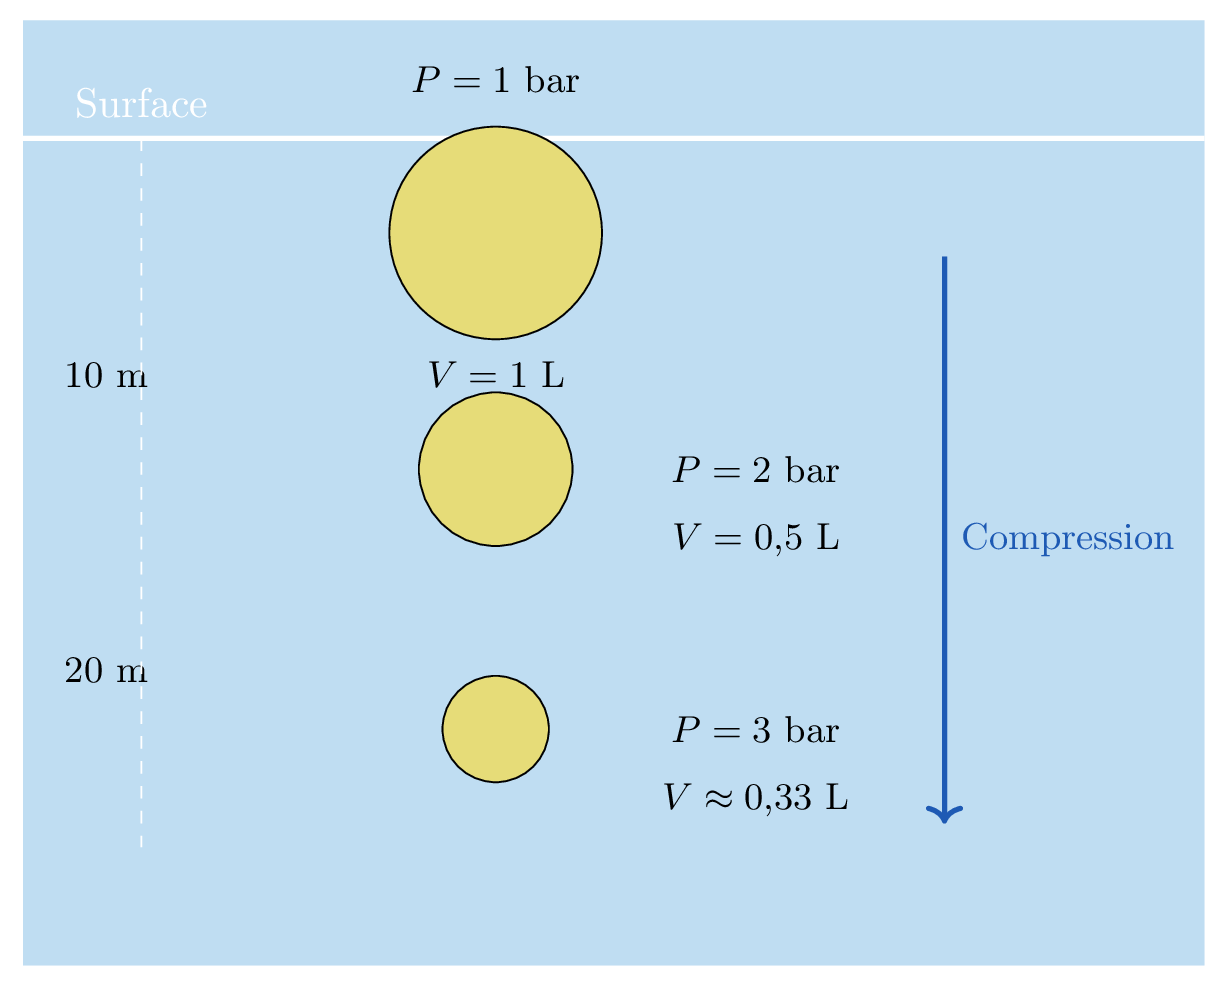
\includegraphics[height=0.6\textheight]{images/ballons_compression}
    \end{column}
  \end{columns}
\end{frame}

\begin{frame}{Conséquences pour le plongeur}

  \begin{block}{À retenir (essentiel)}
    \begin{itemize}
      \item Les espaces remplis d’air se \textbf{compressent} à la descente
            et se \textbf{dilatent} à la remontée.
      \item \alert{Ne jamais bloquer sa respiration à la remontée.}
    \end{itemize}
  \end{block}

  \vspace{0.15cm}

  \begin{block}{Conséquences pratiques}
    \begin{itemize}
      \item À la remontée, \textbf{expirer en continu}, surtout entre
            \textbf{0 et 10 m} (la pression y \textbf{double}).
      \item \textbf{La consommation d’air augmente avec la profondeur}
            (gaz plus dense, pression plus élevée).
      \item \alert{Ne jamais donner de l’air à un plongeur en apnée}
            $\rightarrow$ risque majeur de \textbf{surpression pulmonaire}.
      \item Ces variations expliquent les \textbf{accidents barotraumatiques}
            (oreilles, sinus, masque, dents, poumons).
    \end{itemize}
  \end{block}

\end{frame}

\section{Flottabilité et principe d’Archimède}

\begin{frame}{Principe d’Archimède}
  \begin{block}{Énoncé}
    Tout corps plongé dans un fluide subit une \textbf{poussée verticale de bas en haut}
    égale au \textbf{poids du volume de fluide déplacé}.
  \end{block}

  \begin{itemize}
    \item Deux forces s’opposent :
          \begin{itemize}
            \item le \textbf{poids réel} du plongeur + équipement,
            \item la \textbf{poussée d’Archimède}.
          \end{itemize}
    \item Poids apparent :
          \[
            P_{\text{app}} = P_{\text{réel}} - \text{poussée d’Archimède}
          \]
  \end{itemize}
\end{frame}

\begin{frame}{Exemple de flottabilité}
  \begin{columns}[c]
    \begin{column}{0.6\textwidth}
    \begin{itemize}
      \item Corps de volume 2 L, poids réel 1 kg.
      \item Dans l’eau : volume d’eau déplacé = 2 L $\Rightarrow 2$ kg.
      \item Poids apparent : $1 - 2 = -1$ kg $\Rightarrow$ le corps \textbf{flotte}.
    \end{itemize}

    \begin{block}{Interprétation}
      \begin{itemize}
        \item Poids apparent \textbf{négatif} : flottant.
        \item Poids apparent \textbf{positif} : coule.
        \item Poids apparent \textbf{nul} : équilibre (flottabilité neutre).
      \end{itemize}
    \end{block}
    \end{column}
    \begin{column}{0.4\textwidth}
      \centering
      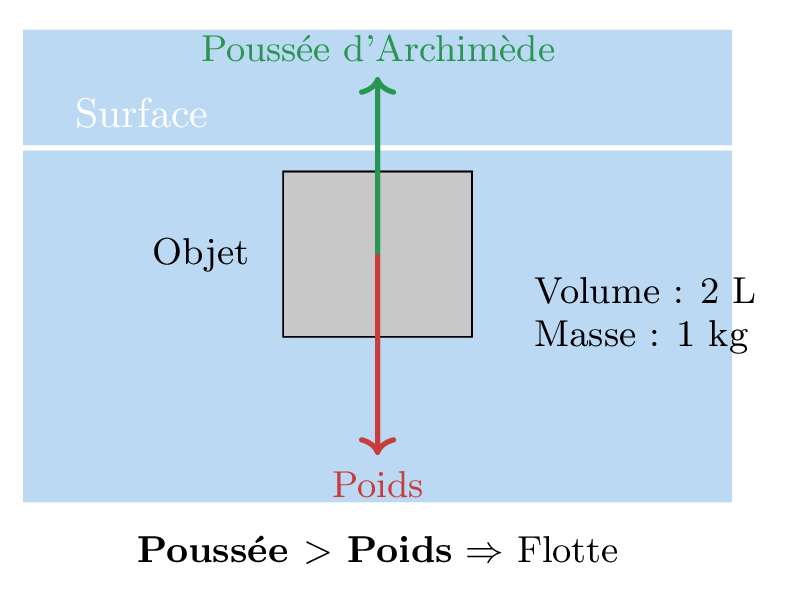
\includegraphics[height=0.5\textheight]{images/flottabilite_archimede}
    \end{column}
  \end{columns}
\end{frame}

\begin{frame}{Application au plongeur}
  \begin{itemize}
    \item Utiliser les \textbf{poumons comme ballast} (inspiration / expiration).
    \item Avoir un \textbf{lestage adapté} à sa morphologie et à l’équipement.
    \item Utiliser un \textbf{gilet stabilisateur} adapté et en bon état.
    \item Objectif : \textbf{flottabilité neutre} en plongée, confortable et sécurisante.
  \end{itemize}
\end{frame}

\section{Accidents barotraumatiques}

\begin{frame}{Principe général}
  \begin{columns}[c]
    \begin{column}{0.5\textwidth}
      \begin{itemize}
        \item Les volumes de gaz se \textbf{compressent} à la descente,
              se \textbf{dilatent} à la remontée (loi de Mariotte).
        \item Si l’air ne peut pas circuler librement, il y a un \textbf{risque de lésion} des tissus.
        \item On parle de \textbf{barotraumatismes}.
      \end{itemize}
    \end{column}
    \begin{column}{0.5\textwidth}
      \centering
      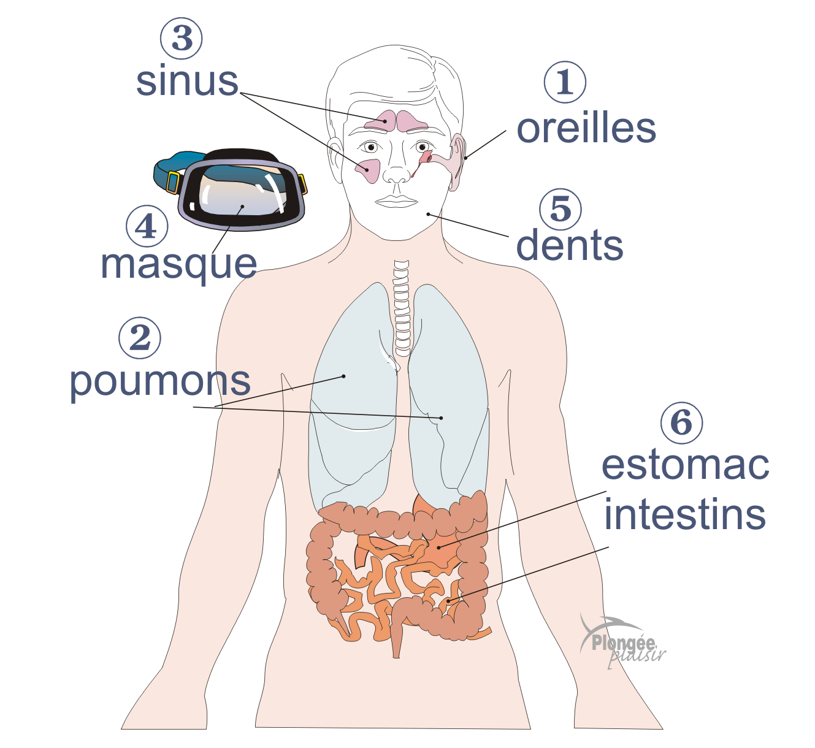
\includegraphics[width=\textwidth]{images/les-6-accidents-barotraumatique}
    \end{column}
  \end{columns}
\end{frame}

\begin{frame}{Plaquage de masque}
  \begin{itemize}
    \item À la descente, l’air dans le masque se \textbf{comprimes}.
    \item La jupe agit comme une \textbf{ventouse} sur le visage et les yeux.
    \item Risques : rougeurs, douleurs, troubles de la vue.
  \end{itemize}
  \begin{block}{Prévention}
    \begin{itemize}
      \item \textbf{Souffler par le nez dans le masque} à la descente.
      \item S’assurer que le masque est bien ajusté mais pas trop serré.
    \end{itemize}
  \end{block}
\end{frame}

\begin{frame}{Dents}
  \begin{block}{Dents}
    \begin{itemize}
      \item Cavités d’air dans une dent mal soignée.
      \item Douleurs à la descente ou à la remontée, risque d’\textbf{éclatement de la dent}.
      \item Prévention : suivi \textbf{régulier chez le dentiste}, arrêter la plongée en cas de douleur persistante.
    \end{itemize}
  \end{block}
\end{frame}

\begin{frame}{sinus}
  \begin{columns}[c]
    \begin{column}{0.45\textwidth}
        \begin{block}{Sinus}
          \begin{itemize}
            \item Cavités osseuses communiquant avec les fosses nasales.
            \item Obstruction $\Rightarrow$ impossibilité d’égaliser la pression.
            \item Douleurs violentes, parfois \textbf{saignements}.
            \item Prévention : ne pas plonger enrhumé, ne jamais forcer, consulter un ORL en cas de problème.
          \end{itemize}
        \end{block}
      \end{column}
    \begin{column}{0.5\textwidth}
      \centering
      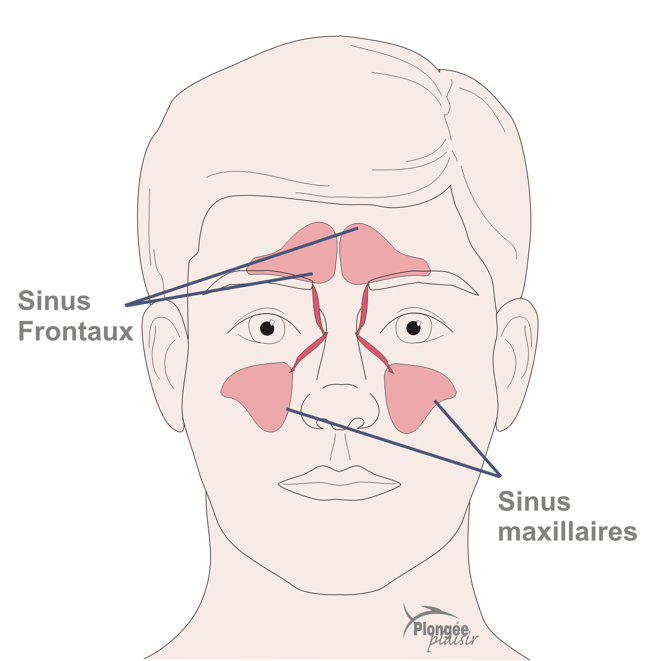
\includegraphics[width=0.9\textwidth]{images/barotraumatisme-sinus}
    \end{column}
  \end{columns}
\end{frame}

\begin{frame}{Oreilles}
  \begin{columns}[c]
    \begin{column}{0.45\textwidth}
      \begin{itemize}
        \item Tympan situé entre oreille externe et oreille moyenne.
        \item À la descente : pression extérieure augmente, tympan repoussé vers l’intérieur.
        \item Si on n’égalise pas : \textbf{douleur}, risque de \textbf{rupture du tympan}.
      \end{itemize}
    \end{column}
    \begin{column}{0.5\textwidth}
      \centering
      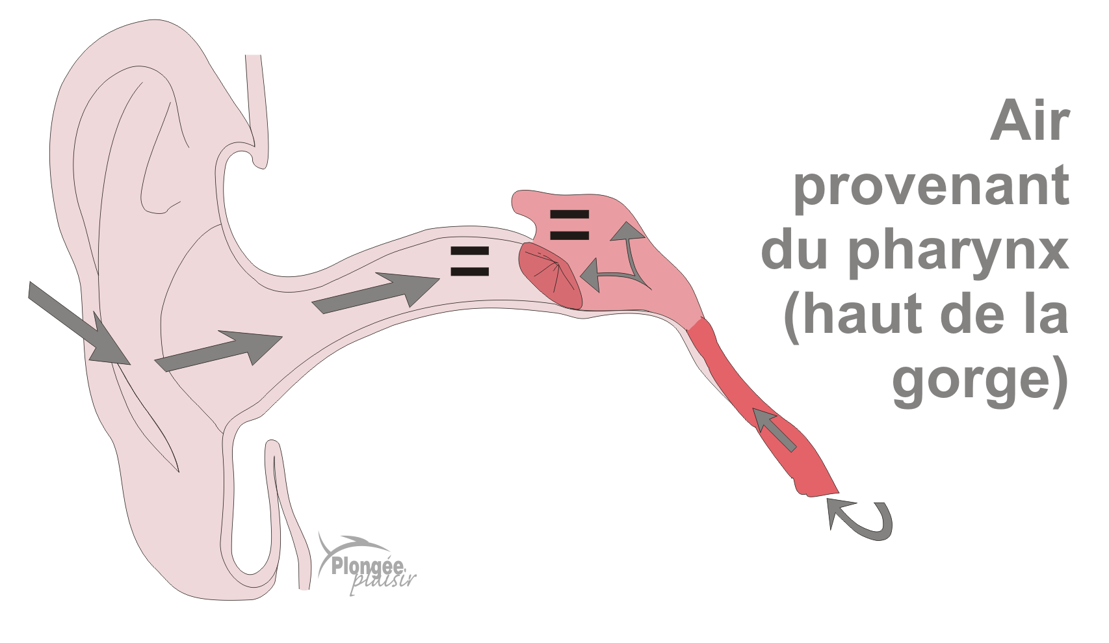
\includegraphics[width=0.9\textwidth]{images/barotraumatisme-oreille}
    \end{column}
  \end{columns}
\end{frame}

\begin{frame}{Manœuvre de Valsalva}
  \begin{block}{Manœuvre de Valsalva}
    \begin{itemize}
      \item Se pincer le nez, bouche fermée, et \textbf{souffler doucement}.
      \item L’air passe par la trompe d’Eustache et rétablit l’équilibre de pression.
      \item À faire \textbf{régulièrement à la descente}, avant la douleur.
      \item \alert{Ne jamais faire de Valsalva à la remontée}.
    \end{itemize}
  \end{block}
  
  \vspace{0.2cm}

  \begin{alertblock}{Attention - conduite à tenir}
    \begin{itemize}
      \item Si, à la descente, une \textbf{douleur survient}, remonter de
            \textbf{quelques mètres} puis redescendre doucement.
      \item \alert{Ne jamais insister}.
      \item Si la douleur persiste : \textbf{consulter un ORL}.
    \end{itemize}
  \end{alertblock}
\end{frame}

\begin{frame}{Coliques du scaphandrier}
  \begin{itemize}
    \item Gaz dans le tube digestif : fermentation des aliments, boissons gazeuses, air avalé.
    \item À la remontée : dilatation des gaz, douleurs abdominales.
  \end{itemize}
  \begin{block}{Prévention}
    \begin{itemize}
      \item Éviter les \textbf{féculents lourds} et les \textbf{boissons gazeuses} avant la plongée.
      \item Manger léger et adapté.
    \end{itemize}
  \end{block}
\end{frame}

\section{Surpression pulmonaire et décompression}

\begin{frame}{Surpression pulmonaire}
  \begin{block}{Définition}
    Lésion des poumons due à une \textbf{dilatation excessive de l’air} contenu dans les alvéoles,
    en cas de \textbf{blocage de la respiration à la remontée}.
  \end{block}

  \begin{itemize}
    \item L’air dans les poumons suit la loi de Mariotte.
    \item Si la remontée se fait \textbf{poumons fermés}, l’air ne peut pas s’échapper.
    \item Risque : \textbf{déchirure des alvéoles} et des vaisseaux sanguins.
    \item Accident de plongée \alert{le plus grave}.
  \end{itemize}
\end{frame}

\begin{frame}{Exemple et zone dangereuse}
  \begin{itemize}
    \item Capacité pulmonaire moyenne : \textbf{5 L}.
    \item À 20 m : $P = 3$ bar. Si on bloque à 20 m et qu’on remonte :
          \[
            3 \times 5 = 1 \times V_{\text{surface}} \Rightarrow V_{\text{surface}} = 15 \text{ L}
          \]
    \item Impossible pour les poumons : lésion bien avant la surface.
  \end{itemize}

  \begin{block}{Zone la plus dangereuse}
    Entre \textbf{0 et 10 m} : la pression est divisée par 2 $\Rightarrow$ le volume d’air est multiplié par 2.
  \end{block}
\end{frame}

\begin{frame}{Prévention de la surpression pulmonaire}
  \begin{columns}[c]
    \begin{column}{0.55\textwidth}
      \begin{alertblock}{Danger majeur}
        Ne jamais bloquer sa respiration à la remontée.
      \end{alertblock}
      \begin{itemize}
        \item Remonter à une \textbf{vitesse maximale de 15 m/min}.
        \item \textbf{Expirer doucement} tout au long de la remontée.
        \item Ne jamais donner d’air à un \textbf{chasseur en apnée}.
      \end{itemize}
    \end{column}
    \begin{column}{0.45\textwidth}
      \centering
      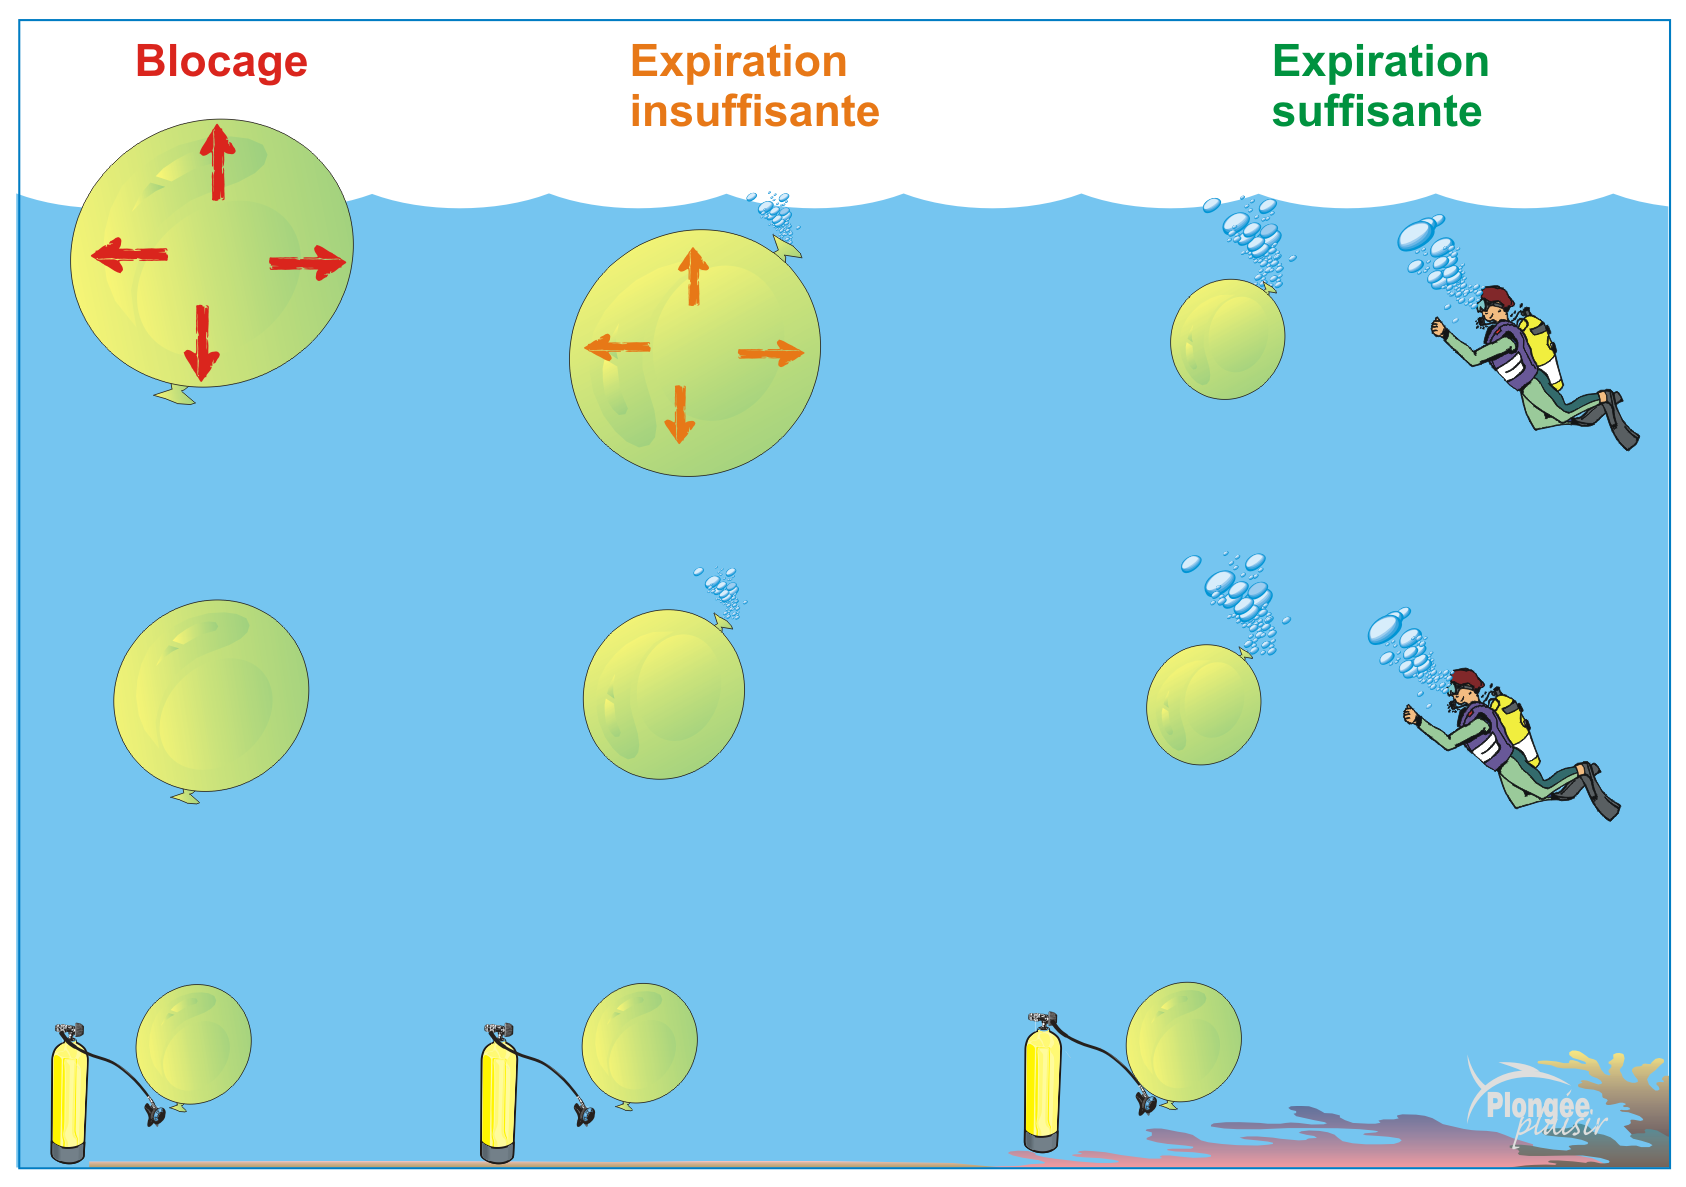
\includegraphics[height=0.6\textheight]{images/barotraumatisme-surpression-pulmonaire}
    \end{column}
    \end{columns}
\end{frame}

\begin{frame}{Accident de décompression}
  \begin{itemize}
    \item Air respiré : \textbf{~80 \% d’azote, ~20 \% d’oxygène}.
    \item L’azote se \textbf{dissout dans l’organisme} en fonction de la profondeur et du temps.
    \item Si la remontée est trop rapide ou les \textbf{paliers non respectés} :
          \begin{itemize}
            \item formation de \textbf{bulles d’azote} dans le sang et les tissus.
          \end{itemize}
  \end{itemize}
\end{frame}

\begin{frame}{Conséquences et prévention}
  \begin{block}{Conséquences possibles}
    \begin{itemize}
      \item Démangeaisons cutanées.
      \item Douleurs ostéo-articulaires.
      \item Atteintes neurologiques, cardiaques, pulmonaires, oreille interne…
    \end{itemize}
  \end{block}

  \begin{block}{Prévention}
    \begin{itemize}
      \item Rester dans la \textbf{courbe de sécurité}.
      \item Respecter la \textbf{vitesse de remontée maximale} 15 m/min et de préférence 10 m/min.
      \item Effectuer les \textbf{paliers obligatoires} et un palier de sécurité
            de \textbf{3 min à 3 m}.
      \item Éviter les efforts importants après la plongée.
      \item Ne pas plonger fatigué.
    \end{itemize}
  \end{block}
\end{frame}

\section{Essoufflement et froid}

\begin{frame}{Essoufflement}
  \begin{itemize}
    \item Comparable à l’essoufflement en course à pied.
    \item Effort trop important + mauvaise ventilation (surtout expiration).
    \item Augmentation du \textbf{CO\textsubscript{2}} $\Rightarrow$ sensation d’oppression, panique possible.
  \end{itemize}

  \begin{block}{Prévention}
    \begin{itemize}
      \item Avoir une \textbf{bonne condition physique}.
      \item Rester \textbf{calme} avant et pendant la plongée.
      \item Produire des \textbf{efforts modérés}.
      \item Ne pas être surlesté.
      \item \textbf{Forcer l’expiration} tout au long de la plongée.
    \end{itemize}
  \end{block}
\end{frame}

\begin{frame}{Reconnaître et signaler l’essoufflement}
  \begin{columns}[c]
    \begin{column}{0.6\textwidth}
      \begin{itemize}
        \item Ventilation \textbf{rapide et superficielle}.
        \item Sentiment de ne plus arriver à reprendre son souffle.
        \item Sentiment d’angoisse possible.
      \end{itemize}

      \begin{block}{Conduite à tenir}
        \begin{itemize}
          \item Faire le signe \og \textbf{je suis essoufflé} \fg{} au guide de palanquée.
          \item Réduire l’effort, se calmer, ventiler lentement et profondément.
        \end{itemize}
      \end{block}
    \end{column}
    \begin{column}{0.4\textwidth}
      \centering
      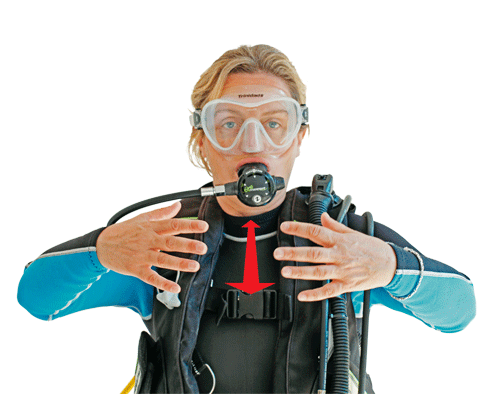
\includegraphics[height=0.5\textheight]{images/signes_essoufflement-2}
    \end{column}
  \end{columns}
\end{frame}

\begin{frame}{Le froid}
  \begin{columns}[c]
    \begin{column}{0.6\textwidth}
      \begin{itemize}
        \item Dans l’eau, le corps se refroidit \textbf{25 fois plus vite} qu’à l’air libre.
        \item Combinaison inadaptée : trop large $\Rightarrow$ circulation d’eau ; trop serrée $\Rightarrow$ gêne la ventilation.
      \end{itemize}
    \end{column}
    \begin{column}{0.4\textwidth}
      \centering
      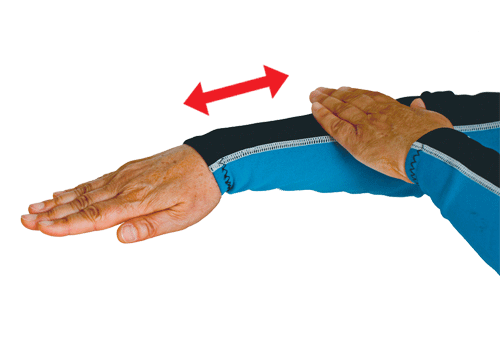
\includegraphics[height=0.4\textheight]{images/signes_froid-2}
    \end{column}
  \end{columns}
  \begin{block}{Prévention}
    \begin{itemize}
      \item Combinaison adaptée à la \textbf{température de l’eau} et à la morphologie.
      \item Alimentation avec \textbf{sucres lents} (repas) et \textbf{sucres rapides} avant la plongée.
      \item Pas d’alcool, éviter de plonger fatigué.
      \item Se couvrir avant et après la plongée.
      \item Signaler le froid : signe \og \textbf{j’ai froid} \fg{}.
    \end{itemize}
  \end{block}
\end{frame}

\section{Tables de plongée et ordinateur}

\begin{frame}{Tables MN90}
    \begin{columns}[c]
    \begin{column}{0.6\textwidth}
      \begin{itemize}
        \item Tables utilisées par la \textbf{FFESSM} : \textbf{MN90}.
        \item Objectif : éviter l'\textbf{accident de décompression}.
        \item Vitesse de remontée : entre \textbf{12 et 15 m/min}.
        \item Paliers à effectuer à la \textbf{profondeur} et pendant le \textbf{temps indiqués}.
      \end{itemize}
    \end{column}
    \begin{column}{0.4\textwidth}
      \centering
      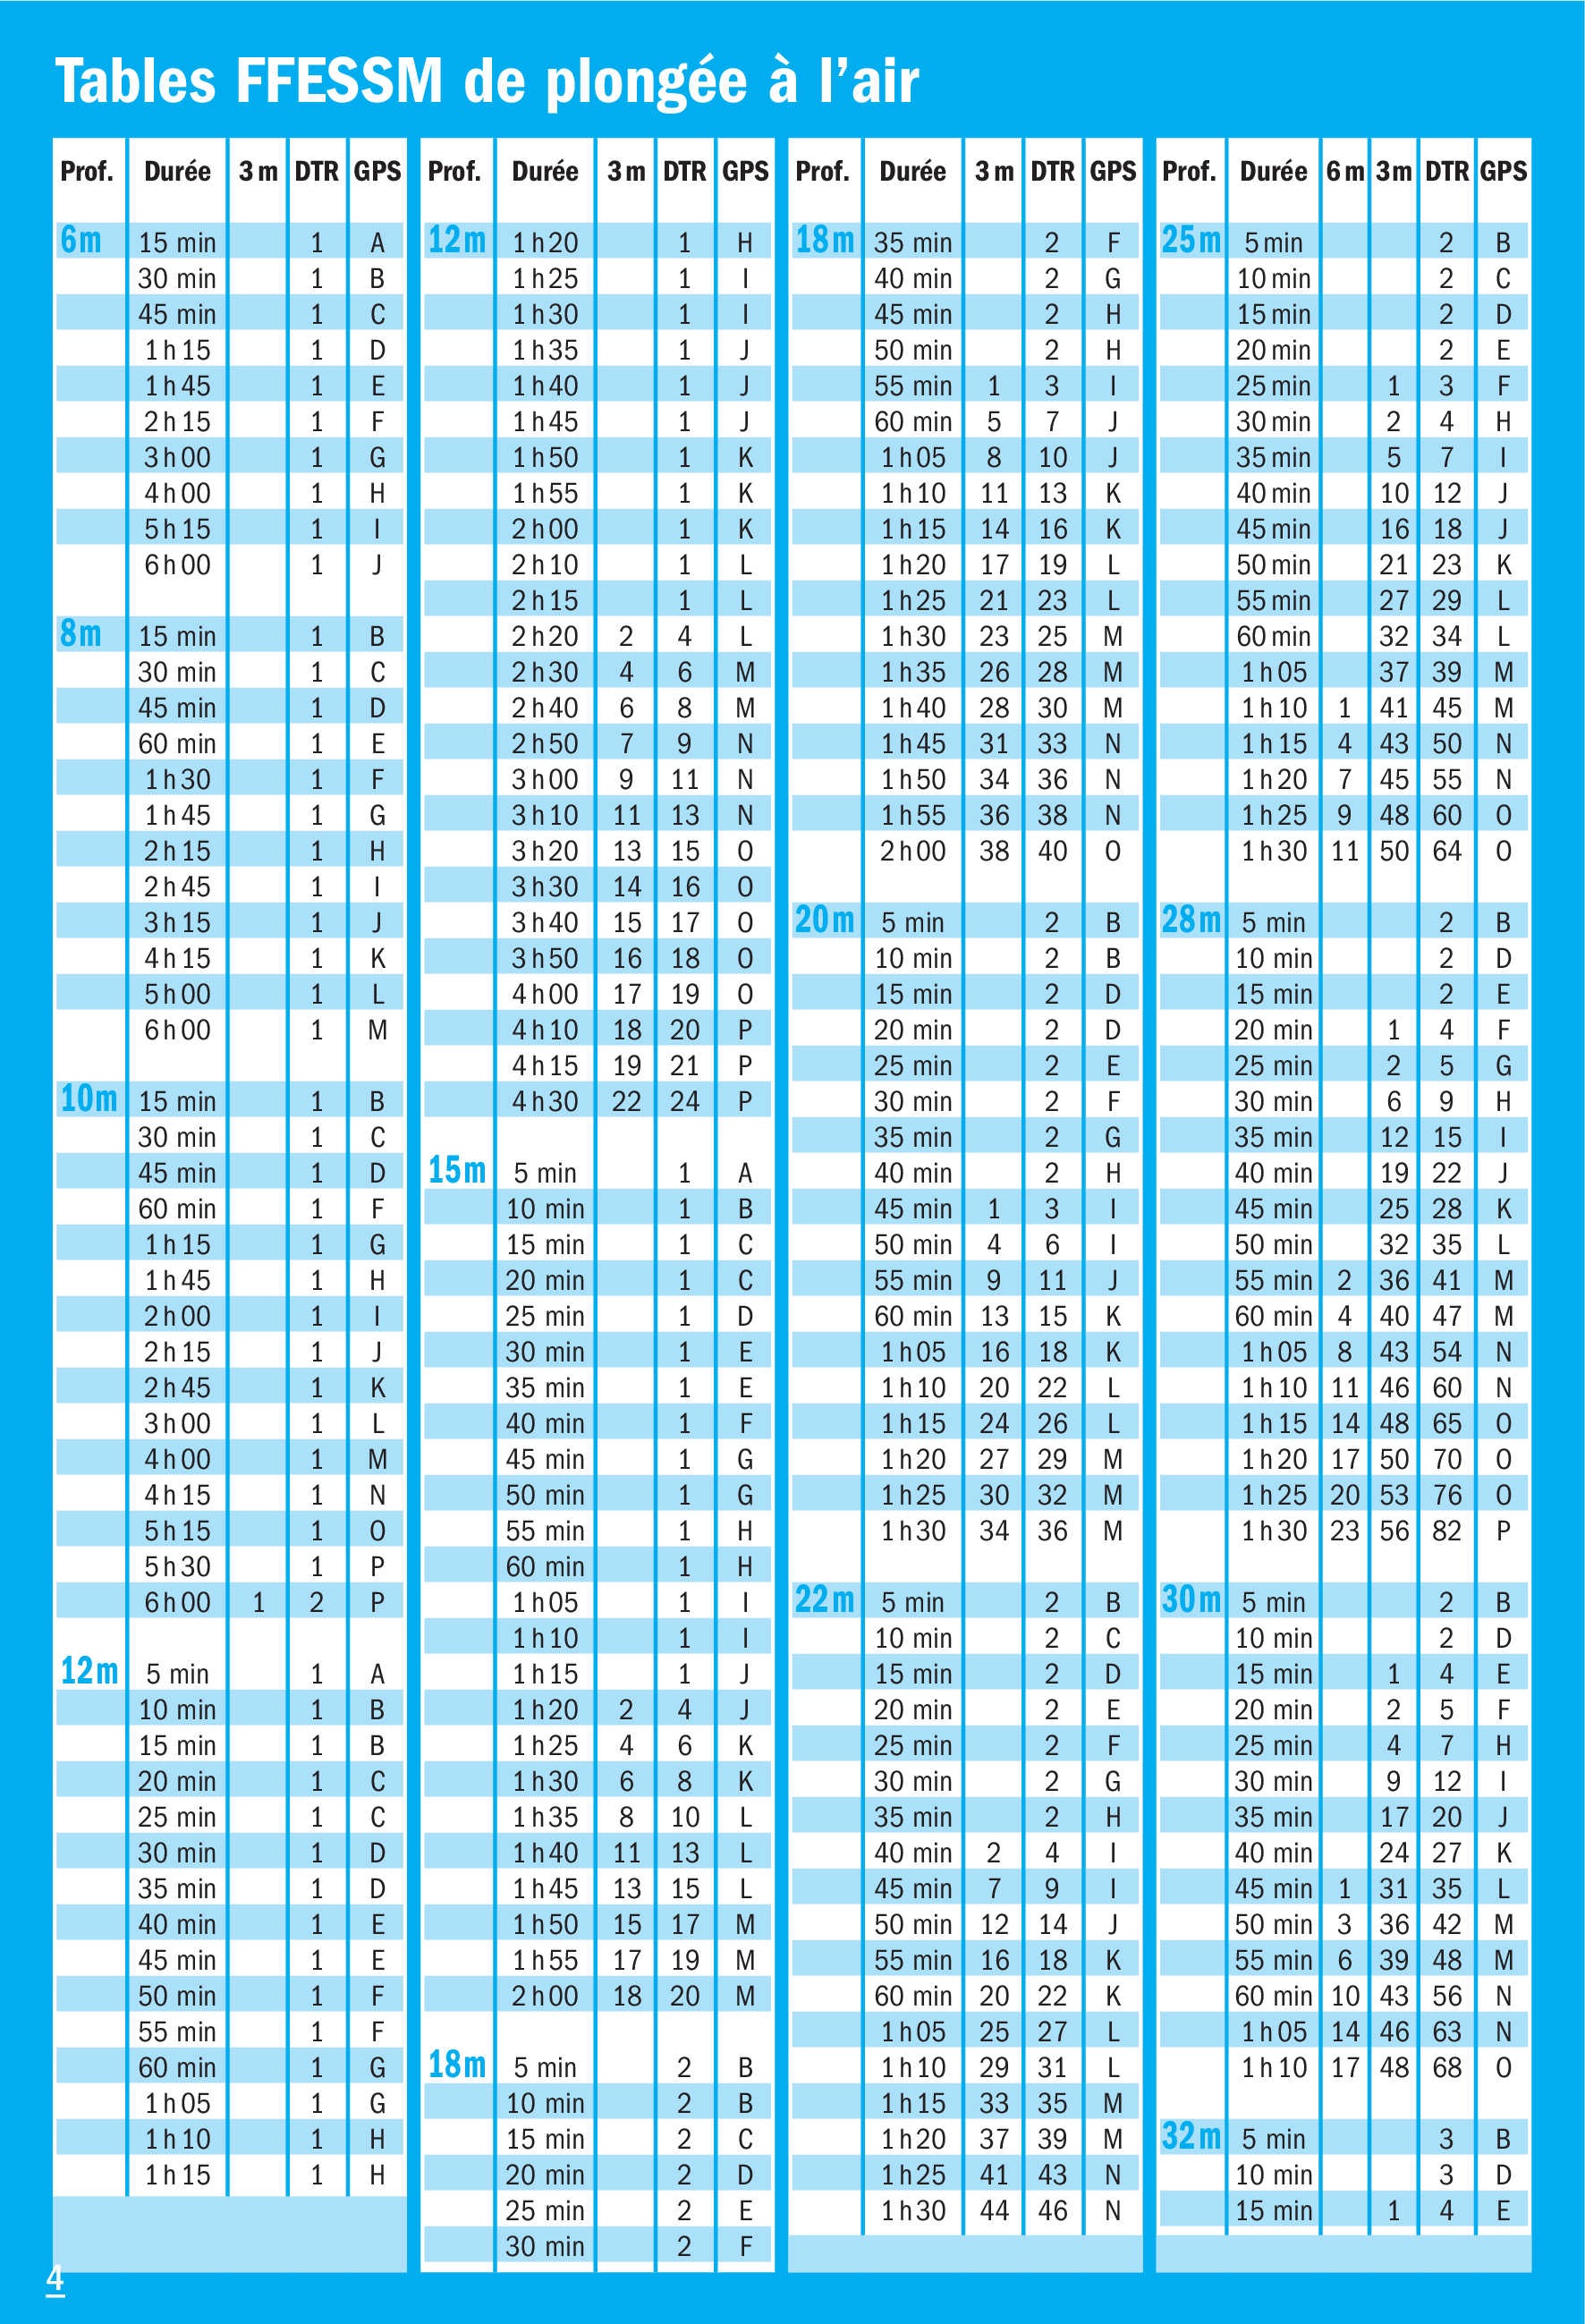
\includegraphics[width=0.79\textwidth]{images/mn90-exemple}
    \end{column}
  \end{columns}
\end{frame}

\begin{frame}{La Courbe de Sécurité}
  \begin{columns}[c]
    \column{0.5\textwidth}
    \textbf{C'est quoi ?}
    \begin{itemize}
      \item Pour chaque \textbf{profondeur}, elle indique le \textbf{temps maxi} de plongée
            possible \textbf{sans palier obligatoire}.
      \item Tant que l'on reste \textbf{sous} cette courbe, on peut remonter directement
            (en respectant la vitesse de remontée).
      \item Si on \textbf{dépasse} ces temps, des \textbf{paliers de décompression} deviennent
            nécessaires.
    \end{itemize}

    \column{0.5\textwidth}
    \centering
    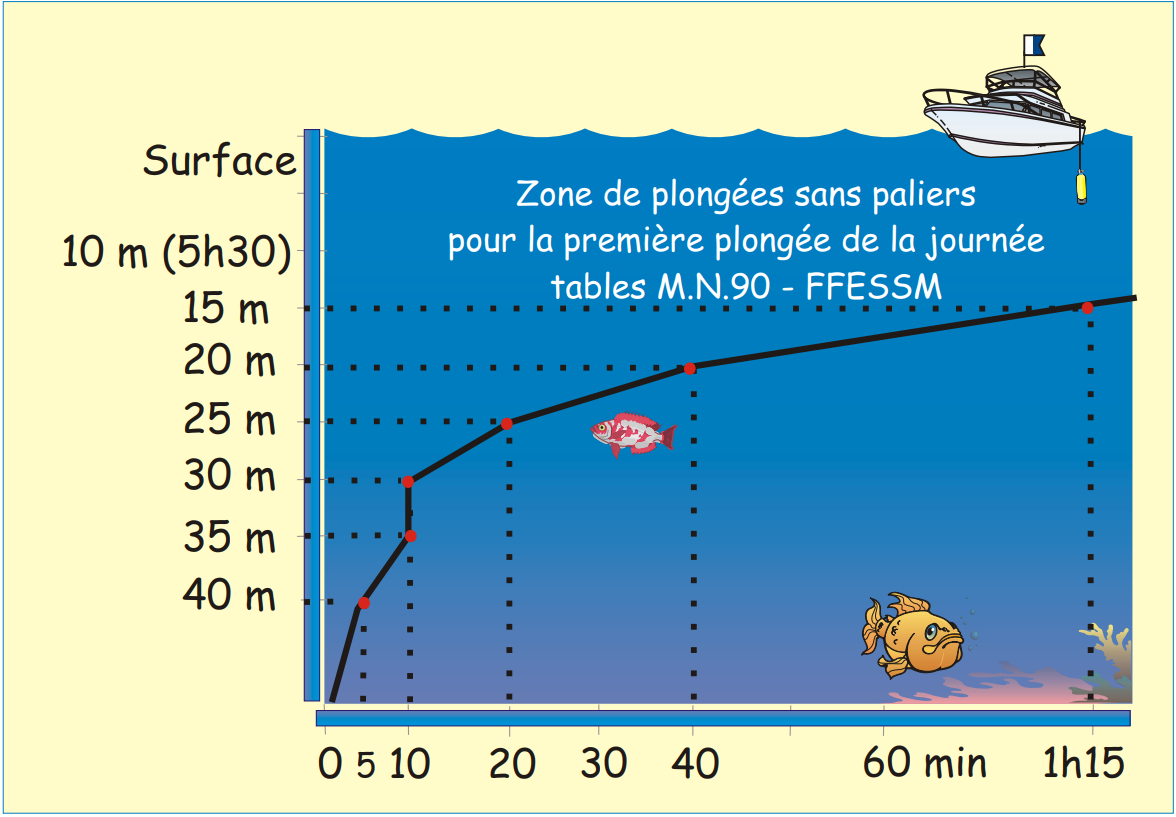
\includegraphics[height=0.6\textheight,keepaspectratio]{images/courbe-de-securite}
  \end{columns}
\end{frame}

\begin{frame}{Ordinateur de plongée}
  \begin{itemize}
    \item Principe identique aux tables mais calcul \textbf{en continu}.
    \item Capteur de pression $\Rightarrow$ profondeur instantanée.
    \item Calcule les \textbf{paliers} en fonction du profil réel.
    \item Indique la \textbf{vitesse de remontée} et les paliers à effectuer.
    \item Mémorise les paramètres pour les plongées suivantes.
  \end{itemize}
\end{frame}

\section{Dangers du milieu et environnement}

\begin{frame}{Dangers liés à la faune}
  \begin{itemize}
    \item Animaux qui \textbf{mordent} : murènes, congres…
    \item Animaux qui \textbf{piquent} : oursins, vives, certaines étoiles de mer, raies…
    \item Animaux qui \textbf{brûlent} : méduses, anémones de mer.
  \end{itemize}

  \begin{block}{Prévention}
    \begin{itemize}
      \item Ne pas \textbf{toucher} les animaux.
      \item Faire attention où l'on \textbf{pose les mains et les genoux}.
      \item Ne pas passer derrière une méduse (filaments parfois très longs).
    \end{itemize}
  \end{block}
\end{frame}

\begin{frame}{Autres dangers du milieu}
  \begin{itemize}
    \item \textbf{Courants} :
          \begin{itemize}
            \item Risque de s'éloigner du bateau.
            \item Nager à contre-courant $\Rightarrow$ essoufflement.
          \end{itemize}
    \item \textbf{Eaux troubles} :
          \begin{itemize}
            \item Risque de perte de la palanquée.
            \item Rester \textbf{regroupés côte à côte}.
          \end{itemize}
    \item \textbf{Grottes, tunnels, épaves} :
          \begin{itemize}
            \item Visibilité réduite, risque de rester coincé.
            \item Ne pas enlever son masque dans les grottes.
            \item Ne pas rentrer dans les épaves.
          \end{itemize}
    \item \textbf{Filets, cordages} :
          \begin{itemize}
            \item Risque d'emmêlement.
            \item Ne pas se débattre, appeler le coéquipier.
          \end{itemize}
  \end{itemize}
\end{frame}

\begin{frame}{Embarcations et parachute}
  \begin{itemize}
    \item Risque de \textbf{collision} avec des bateaux.
    \item Toujours regarder (360°) et écouter avant de faire surface.
    \item Le \textbf{parachute de palier}, géré par le guide, est un élément de sécurité.
  \end{itemize}
\end{frame}

\begin{frame}{Protection de l'environnement}
  \begin{itemize}
    \item L'écosystème sous-marin est \textbf{fragile}.
    \item Ne pas \textbf{palmer en raclant le fond} : les palmes sont l'ennemi n°1 de la faune et de la flore.
    \item Ne pas arracher coraux, gorgones, etc.
    \item Regarder, mais \textbf{ne pas toucher}.
    \item Ne pas perturber les animaux, surtout en période de reproduction.
    \item Ne tuer aucun animal : nous sommes des \textbf{invités} dans ce milieu.
  \end{itemize}
\end{frame}

\begin{frame}{Sons, couleurs et dimensions sous l'eau}
  \begin{columns}
    \column{0.5\textwidth}
    \begin{itemize}
      \item \textbf{Sons} :
        \begin{itemize}
          \item Ils se propagent plus vite dans l'eau.
          \item \textbf{Difficile de localiser} la provenance (avant / arrière, gauche / droite).
        \end{itemize}
      \item \textbf{Couleurs} :
        \begin{itemize}
          \item Le rouge disparaît dès \textbf{5–10 m}, puis l'orange, le jaune, etc.
          \item Tout paraît plus \textbf{bleu / vert} avec la profondeur.
        \end{itemize}
      \item \textbf{Dimensions} :
        \begin{itemize}
          \item Les objets paraissent \textbf{plus gros et plus proches} (effet masque + eau).
          \item Attention à l'\textbf{estimation des distances} et des tailles.
        \end{itemize}
    \end{itemize}

    \column{0.5\textwidth}
    \centering
    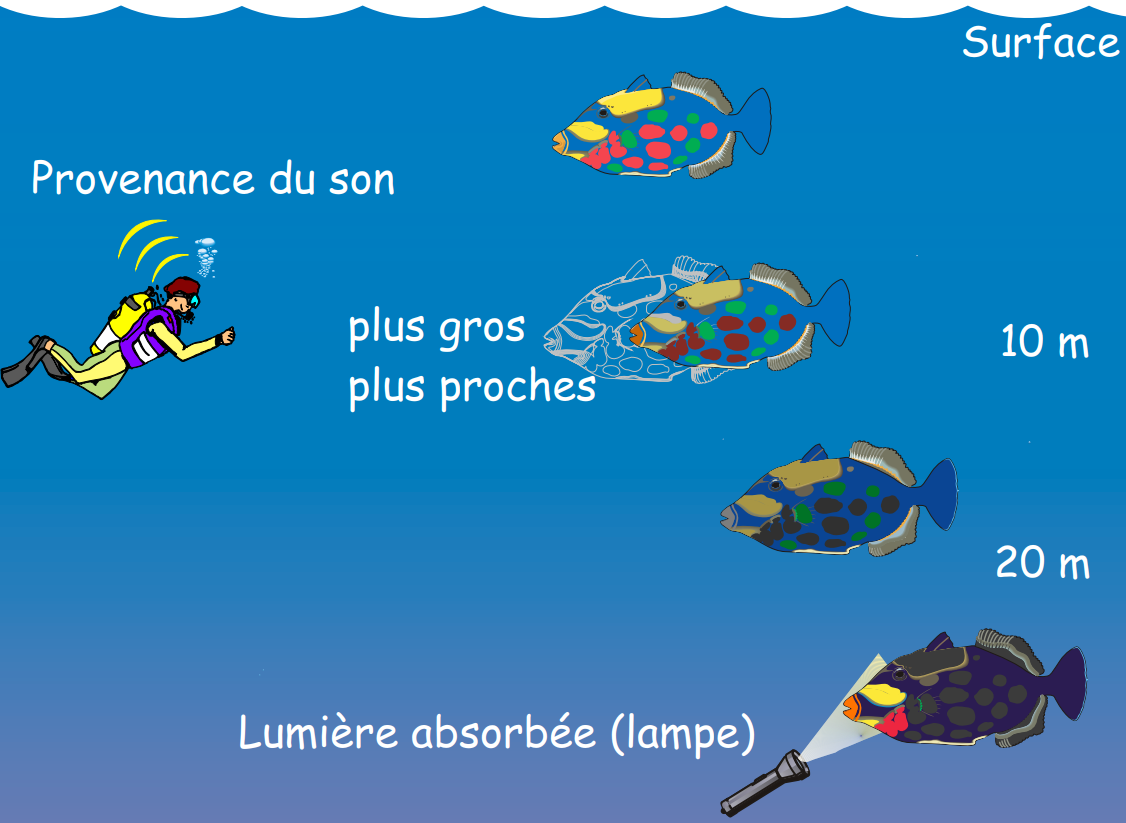
\includegraphics[width=\columnwidth,keepaspectratio]{images/sons-couleurs-dimensions}
  \end{columns}
\end{frame}

\section{Signes et communication}

\begin{frame}{Importance des signes}
  \begin{itemize}
    \item Sous l’eau, on ne parle pas : les \textbf{signes manuels} sont le seul moyen sûr de communication.
    \item Ils doivent être \textbf{amples, clairs et sans ambiguïté}.
    \item Permettent de transmettre rapidement :
          \begin{itemize}
            \item un \textbf{problème},
            \item une \textbf{information},
            \item un \textbf{ordre de sécurité}.
          \end{itemize}
  \end{itemize}
\end{frame}

\begin{frame}{Signes de base (exemples)}
  \centering
  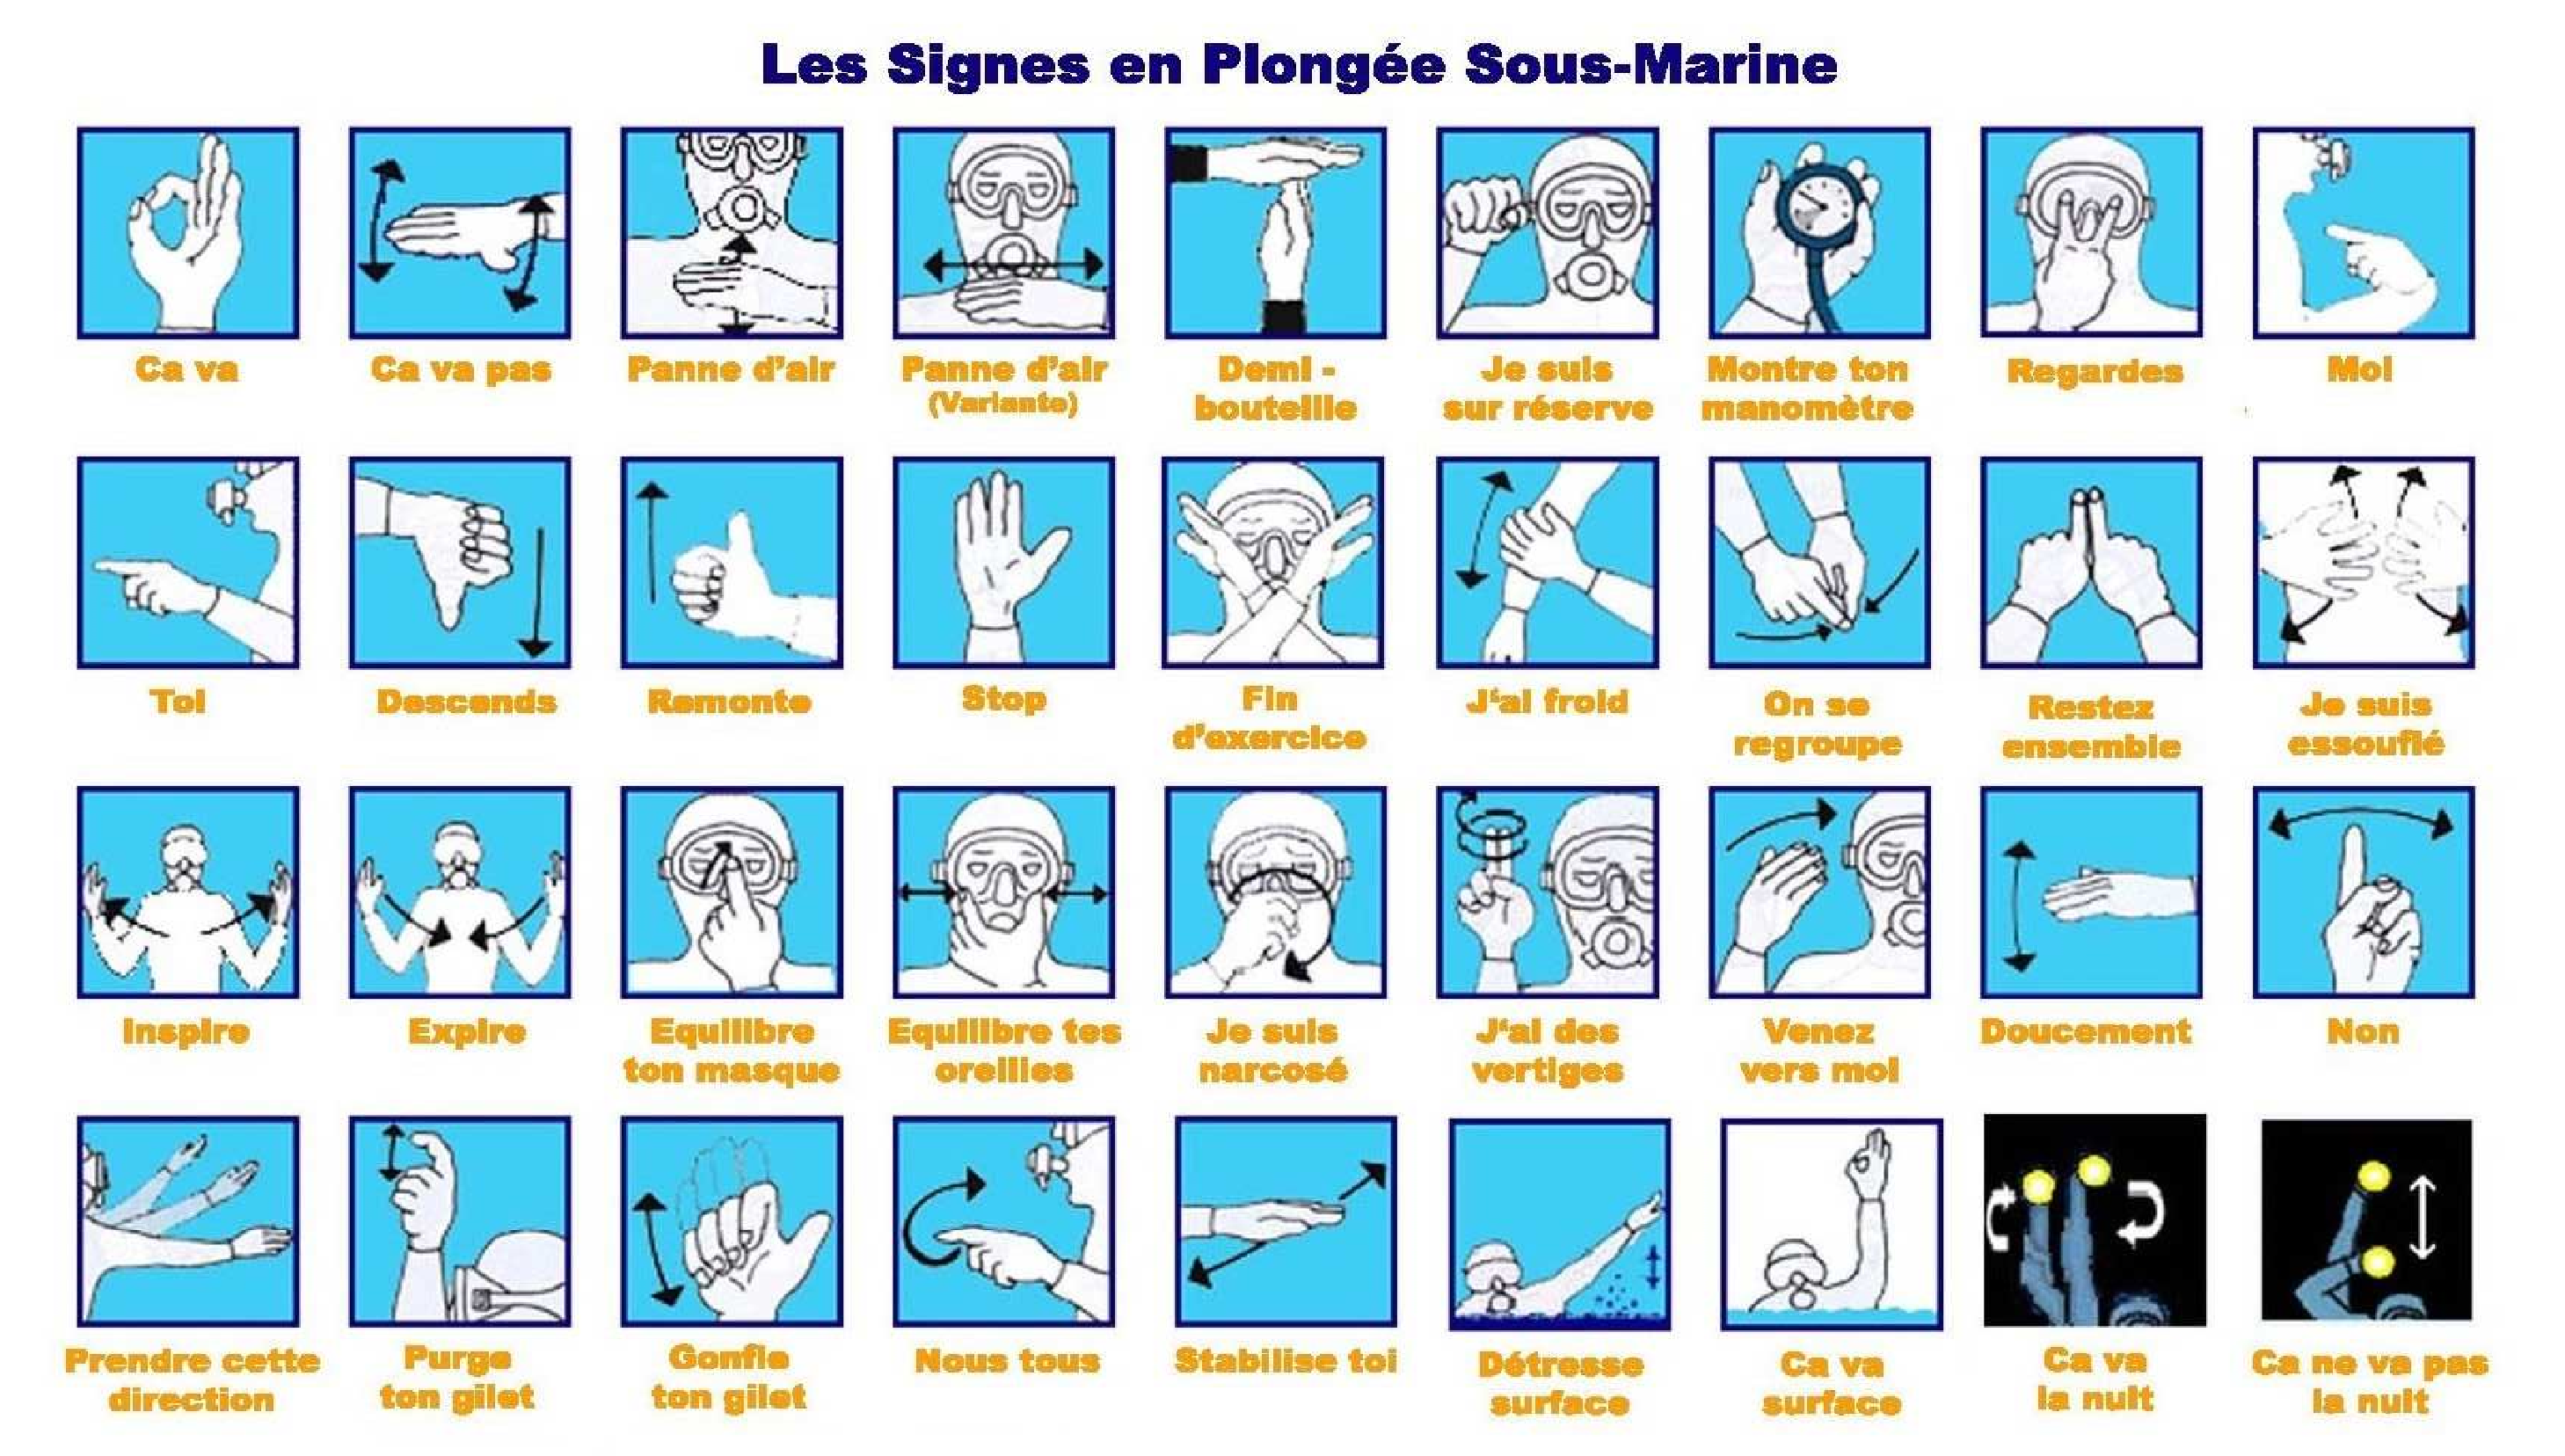
\includegraphics[width=0.79\textwidth]{images/signes_communication}
\end{frame}

\section{Les règles de sécurité}

\begin{frame}{Les règles de sécurité}
  \begin{block}{Principe général}
    \begin{itemize}
      \item La plongée est une activité de loisir, qui se pratique
            dans le respect strict des règles de sécurité.
      \item Ces règles s’appliquent \textbf{avant, pendant et après la plongée}.
    \end{itemize}
  \end{block}
\end{frame}

\begin{frame}{Avant la plongée}
\begin{itemize}
  \item \alert{Ne jamais plonger si on n’en a pas envie}
        (fatigue, traitements médicaux, affections ORL, gueule de bois…).
  \item Contrôler son matériel :
        \begin{itemize}
          \item pression de la bouteille,
          \item fonctionnement du détendeur,
          \item présence de la ceinture de lest,
          \item gilet et direct system.
        \end{itemize}
  \item Écouter les consignes du \textbf{directeur de plongée}
        et de son \textbf{guide de palanquée}.
  \item \alert{Ne jamais plonger seul}.
\end{itemize}
\end{frame}

\begin{frame}{Mise à l’eau et descente}
\begin{block}{Mise à l’eau}
\begin{itemize}
  \item Le guide de palanquée se met à l’eau en premier.
  \item Gonfler le gilet en surface.
  \item Rester groupé avec tous les membres de sa palanquée.
\end{itemize}
\end{block}

\vspace{0.2cm}

\begin{block}{À la descente}
\begin{itemize}
  \item Descendre uniquement sur ordre du guide de palanquée.
  \item \alert{Ne jamais descendre plus bas que son guide de palanquée}.
  \item Stopper la descente en cas de douleur
        (sinus, oreilles, estomac).
\end{itemize}
\end{block}
\end{frame}

\begin{frame}{Pendant la plongée}
\begin{itemize}
  \item Ne jamais se laisser tenter par la profondeur.
  \item Si un plongeur fait le signe \textbf{« réserve »},
        \alert{toute la palanquée remonte}.
  \item Signaler au guide de palanquée que vous êtes en réserve.
  \item Signaler tout évènement au guide de palanquée.
  \item En cas de perte de la palanquée :
        \begin{itemize}
          \item attendre \textbf{1 minute},
          \item puis remonter à \textbf{10 m/min},
          \item et retour en surface.
        \end{itemize}
\end{itemize}
\end{frame}

\begin{frame}{Remontée et surface}

\begin{block}{À la remontée}
\begin{itemize}
  \item \alert{Ne jamais bloquer sa respiration}.
  \item Ne jamais remonter plus vite que son guide de palanquée.
  \item Respecter la vitesse de remontée de \textbf{10 m/min}
        et les paliers.
  \item Regarder (360°) et écouter avant de faire surface.
\end{itemize}
\end{block}

\vspace{0.2cm}

\begin{block}{En surface}
\begin{itemize}
  \item Attendre toute la palanquée pour rejoindre le bateau.
  \item Attendre que l’échelle soit dégagée.
  \item \alert{Ne pas rester sous l’échelle}.
\end{itemize}
\end{block}
\end{frame}

\begin{frame}{Règles de sécurité — Après la plongée}

\begin{itemize}
  \item Écouter le briefing du guide de palanquée.
  \item \alert{Signaler toute sensation inhabituelle} :
        fatigue, nausée, picotements, malaise…
  \item Ne pas prendre l’avion dans les \textbf{12 à 24 heures}
        suivant la plongée.
  \item Ne pas faire d'effort physique intense
        dans les \textbf{6 heures} suivant la plongée.
  \item Ne pas faire de l'apnée dans les \textbf{6 heures} suivant la plongée.
\end{itemize}
\end{frame}

\section{Questions et conclusion}

\begin{frame}{Questions / échanges}
  \centering
  \Large
  Des questions ?\\[0.5cm]
  \normalsize
  N’hésitez pas à revenir sur :
  \begin{itemize}
    \item les notions de \textbf{pression} et de \textbf{flottabilité},
    \item les \textbf{accidents barotraumatiques},
    \item la \textbf{surpression pulmonaire} et la \textbf{décompression},
    \item les \textbf{règles de sécurité} qui vous semblent importantes.
  \end{itemize}
\end{frame}

\begin{frame}{Pour finir...}
  \begin{itemize}
    \item La plongée est un \textbf{sport magnifique} mais potentiellement dangereux.
    \item Le respect des \textbf{règles de sécurité} permet de garder le \textbf{plaisir} au centre.
    \item La théorie N1 est là pour vous donner les \textbf{bases indispensables}.
  \end{itemize}

  \vfill
  \centering
  \Large
  \textbf{Bonnes plongées !!!}
\end{frame}


\end{document}
